% file: graphs_v5_rep_5_3.tex
% created by Orbiter tikz interface
% creation date: Sat Jul 30 08:11:07 +03 2022
% DeviceCoordinates 0 0 1000000 1000000
% UserCoordinates 0 0 10000 10000
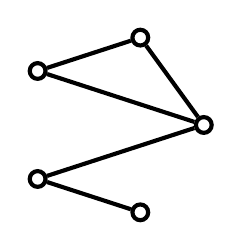
\begin{tikzpicture}[scale=0.1,line width = 1.5pt]
\draw [] (28.3333,16.6667) -- (20.27,27.76);
\draw [] (28.3333,16.6667) -- (7.23,23.5233);
\draw [] (28.3333,16.6667) -- (7.23,9.81);
\draw [] (20.27,27.76) -- (7.23,23.5233);
\draw [] (7.23,9.81) -- (20.27,5.57333);
\filldraw[color=white] (28.3333,16.6667) circle [radius = 1cm];
\draw (28.3333,16.6667) circle [radius = 1cm];
\filldraw[color=white] (20.27,27.76) circle [radius = 1cm];
\draw (20.27,27.76) circle [radius = 1cm];
\filldraw[color=white] (7.23,23.5233) circle [radius = 1cm];
\draw (7.23,23.5233) circle [radius = 1cm];
\filldraw[color=white] (7.23,9.81) circle [radius = 1cm];
\draw (7.23,9.81) circle [radius = 1cm];
\filldraw[color=white] (20.27,5.57333) circle [radius = 1cm];
\draw (20.27,5.57333) circle [radius = 1cm];
\end{tikzpicture}
